\documentclass{article}
\usepackage{graphicx,subfig}
\usepackage{graphicx,fancyhdr,amsmath,amssymb,amsthm,subfig,url,hyperref}
\usepackage[margin=1in]{geometry}
\usepackage{subfig}
\usepackage[utf8]{inputenc}
\usepackage{hyperref}
\usepackage{amsmath}
\usepackage{listings}
\usepackage{xcolor} % for customizing colors (optional)
\DeclareUnicodeCharacter{2212}{-}
%\DeclareUnicodeCharacter{2265}{≥}
% \DeclareUnicodeCharacter{2264}{$\leq$}
% \DeclareUnicodeCharacter{2265}{$\beq$}
%----------------------- Macros and Definitions --------------------------
%%% FILL THIS OUT
\lstset{
    language=Matlab, % set language to MATLAB
    basicstyle=\ttfamily\small, % font type and size
    numbers=left, % line numbers on the left
    numberstyle=\tiny, % style of the line numbers
    stepnumber=1, % display every line number
    frame=single, % frame around the code block
    backgroundcolor=\color{gray!10}, % background color
    keywordstyle=\color{blue}, % color for MATLAB keywords
    commentstyle=\color{green!50!black}, % color for comments
    stringstyle=\color{red}, % color for strings
    breaklines=true, % line breaking
    breakatwhitespace=true % break lines only at whitespaces
}
\newcommand{\SecondAuther}{Mohammad Parsa Dini - std id: 400101204}
\newcommand{\exerciseset}{Computer Homework 2 (Report)}
%%% END
\renewcommand{\theenumi}{\bf \Alph{enumi}}
%\theoremstyle{plain}
%\newtheorem{theorem}{Theorem}
%\newtheorem{lemma}[theorem]{Lemma}
\fancypagestyle{plain}{}
\pagestyle{fancy}
\fancyhf{}
\fancyhead[RO,LE]{\sffamily\bfseries\large Sharif University of Technology}
\fancyhead[LO,RE]{\sffamily\bfseries\large EE 25-851: Graph Signal Processing}
\fancyfoot[LO,RE]{\sffamily\bfseries\large Computer Homework 2}
\fancyfoot[RO,LE]{\sffamily\bfseries\thepage}
\renewcommand{\headrulewidth}{1pt}
\renewcommand{\footrulewidth}{1pt}
\newcommand{\circledtimes}{\mathbin{\text{\large$\bigcirc$}\kern-0.9em\times}}
\graphicspath{{figures/}}
%-------------------------------- Title ----------------------------------
\title{
    
\includegraphics[width=3cm]{logo.png} \\ % Adjust width as needed
    Graph Signal Processing \par \exerciseset
}
\author{\SecondAuther }
%--------------------------------- Text ----------------------------------
\begin{document}
\maketitle
\section*{Problem 1}
\begin{enumerate}
    \item First of all, this is the adjacency matrix of graph $G$:
    \begin{equation*}
        W = 
        \begin{bmatrix}
        0 & 1 & 1 & 0 & 0 & 0 & 0 & 1 \\
        1 & 0 & 1 & 1 & 1 & 0 & 0 & 1 \\ 
        1 & 1 & 0 & 1 & 0 & 0 & 0 & 0 \\ 
        0 & 1 & 1 & 0 & 1 & 1 & 0 & 1 \\ 
        0 & 1 & 0 & 1 & 0 & 1 & 1 & 1 \\ 
        0 & 0 & 0 & 1 & 1 & 0 & 1 & 0 \\ 
        0 & 0 & 0 & 0 & 1 & 1 & 0 & 0 \\ 
        1 & 1 & 0 & 1 & 1 & 0 & 1 & 0 \\ 
        \end{bmatrix}
    \end{equation*}.
    and also here's the graph:
    \begin{figure}[h!]
        \centering
        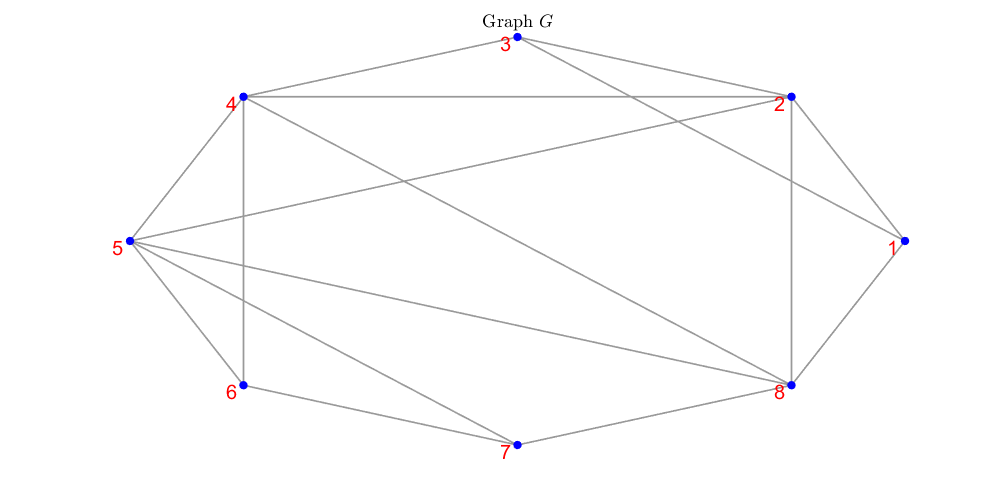
\includegraphics[scale=0.4]{graph_gg.png} 
        \caption{The graph $G$}
        \label{fig:gr1}
    \end{figure}
    % ----------------------------
    \item Here is ho we define the signal $x= 2u_1 + u_2$:
\begin{lstlisting}
G = gsp_compute_fourier_basis(G);     % computing the fourier basis
U12 = G.U(:, 1:2);                    % the 1st and 2nd components of U
x = 2*U12(:,1) + U12(:,2);            % defining the signal x
x_n = awgn(x, 10);                    % adding white gaussian noise
snr_n = db(snr(x_n, x));              % getting the snr 
\end{lstlisting}
    The signals are depicted down below are the signals $x$ and its noisy version $x_n$ in time domain:
    
    \begin{figure}[h!]
        \centering
        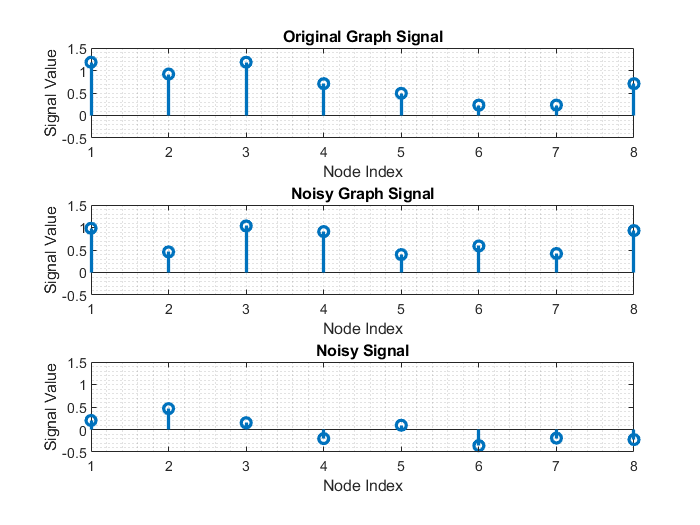
\includegraphics[scale=0.4]{fig6.png} 
        \caption{The graph signals $x$ , $x_n$ time representation with respect to shift operators $W_N$ and $L_N$}
        \label{fig:gr3}
    \end{figure}
    % ---------------
    \item The signals are depicted down below are the  Fourier representations of signals $x$ and its noisy version $x_n$:

     \begin{figure}[h!]
        \centering
        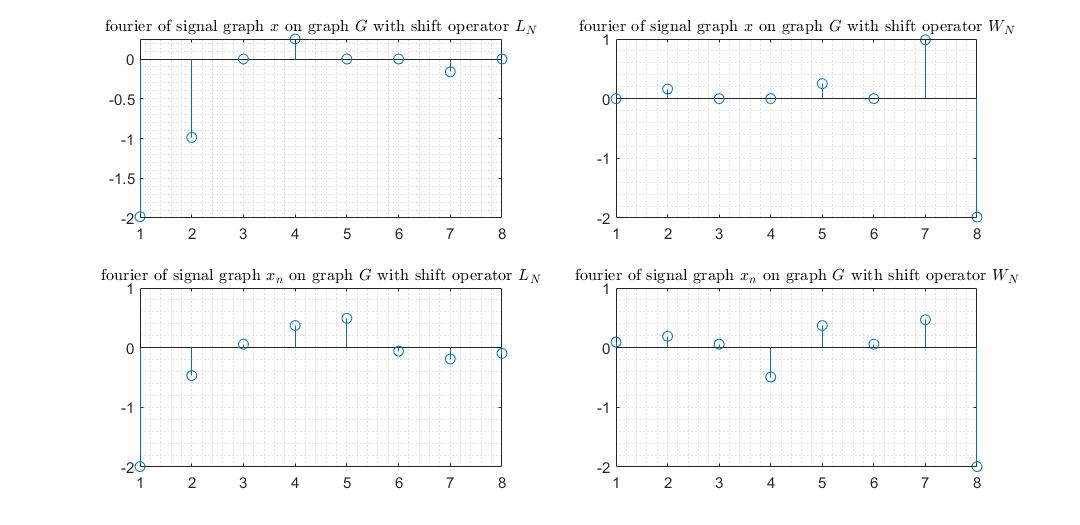
\includegraphics[scale=0.4]{fig7.png} 
        \caption{The graph signals $x$ , $x_n$ fourier representation with respect to shift operators $W_N$ and $L_N$}
        \label{fig:gr4}
    \end{figure}
    % ---------------
    \item Now that we have $W_N = D^{-\frac{1}{2}} W  D^{-\frac{1}{2}}$ and also $L_N =  D^{-\frac{1}{2}} (D - W)  D^{-\frac{1}{2}}$ as shift operators, we assign $h_{\text{filter},L_N} = \text{diag}([1, 1, 0, 0, 0, 0, 0, 0])$ and $h_{\text{filter},W_N} = \text{diag}([0, 0, 0, 0, 0, 0, 1, 1])$ as the filter for the signals based on normalized laplacian and normalized weight matrix, respectively. They are designed as such that they choose the first two components of low-frequent components. These components are the first two components of Laplacian matrix whereas the last two components of weight matrix.
    \newpage
    
    \begin{figure}[h!]
        \centering
        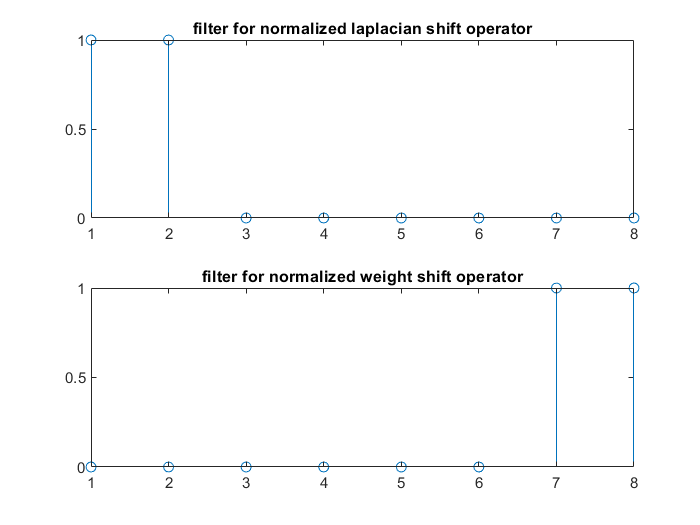
\includegraphics[scale=0.5]{fig8.png} 
        \caption{The  filters $h_{\text{filter},L_N}$ and 
        $h_{\text{filter},W_N}$ 
        }
        \label{fig:gr5}
    \end{figure}
    \item 
    Here is the code for getting the basis based on the shift operator, getting its fourier transform and then apply the filter and the apply an inverse fourier transform:

\begin{lstlisting}
[U_lap, e_lap] = eig(L_N);
Lambda1 = diag(e_lap);
Gn.L = L_N;
Gn = gsp_compute_fourier_basis(Gn);

W_N = D^(-1/2) * W * D^(-1/2);
H = gsp_graph(W_N);
H = gsp_compute_fourier_basis(H);
[U_wn, e_wn] = eig(W_N);
Lambda2 = diag(e_wn);

Filter_H_L = [1 1 0 0 0 0 0 0];
x_n_hat_L = (U_lap)' *x_n;
y_hat_L = diag(Filter_H_L)* x_n_hat_L;
y_L = (U_lap)* y_hat_L;

Filter_H_W = [0 0 0 0 0 0 1 1];
x_n_hat_W = (U_wn)' *x_n;
y_hat_W = diag(Filter_H_W)* x_n_hat_W;
y_W = (U_wn)* y_hat_W;
\end{lstlisting}

    And the results of filtered signals are depicted down below:

    \newpage
    
    \begin{figure}[h!]
        \centering
        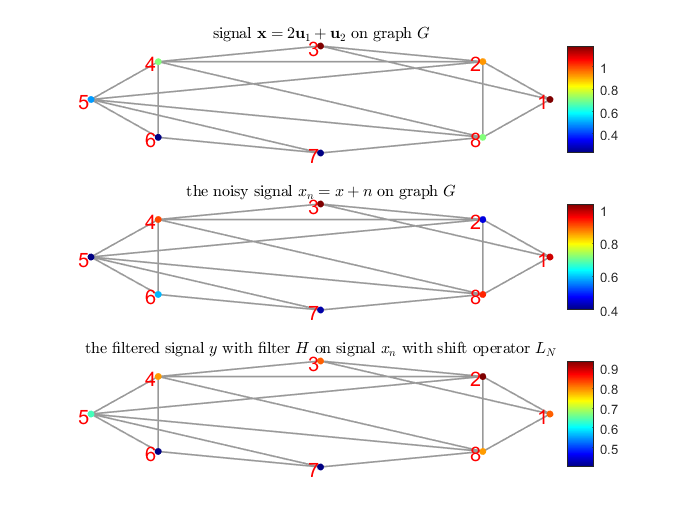
\includegraphics[scale=0.4]{fig4.png} 
        \caption{The graph signal $x_n$ after being filtered by $h_{\text{filter},L_N}$}
        \label{fig:gr5}
    \end{figure}
    \begin{figure}[h!]
        \centering
        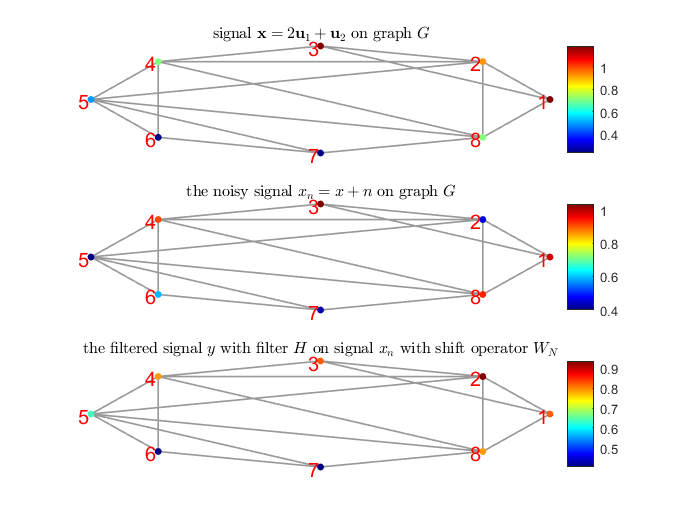
\includegraphics[scale=0.4]{fig5.png} 
        \caption{The graph signal $x_n$ after being filtered by $h_{\text{filter},W_N}$}
        \label{fig:gr5}
    \end{figure}

    % -------------------------------
    \item We calculate the SNR of both filters as below (It seems both have the same performance over retrieving the signal $x$):

\begin{lstlisting}

noise_component_L = y_L - x; 
filtered_noise_power_L = sum(noise_component_L.^2) / length(noise_component_L); 
snr_filtered_L = 10 * log10(signal_power / filtered_noise_power_L);

noise_component_W = y_W - x; 
filtered_noise_power_W = sum(noise_component_W.^2) / length(noise_component_W); 
snr_filtered_W = 10 * log10(signal_power / filtered_noise_power_W);

if snr_filtered_W > snr_filtered_L
    disp('The $W_N$ matrix outperforms with respect to $L_N$');
elseif snr_filtered_W == snr_filtered_L
    disp('Both matrices have the same performance');
else
    disp('The $L_N$ matrix outperforms with respect to $W_N$');
end
disp(snr_filtered_L);
disp(snr_filtered_W);
-------
>> Both matrices have the same performance
>>   11.4358

>>   11.4358
\end{lstlisting}
    % -----
    \item 
    We consider the MSE metric for  the error in order to get both signals close  to each other:
    \begin{align*}
    \|x_\text{ideal} - x_\text{fir}\|_2 &= \|\hat{x}_\text{ideal} - \hat{x}_\text{fir}\|_2 \\
    &= \|\hat{x}\|_2 \cdot \|h_\text{ideal} - h_\text{fir}\|_2 \\
    &\implies h_\text{fir,opt} = \arg\min_{h \in \text{FIR}} \|h_\text{ideal} - h\|_2
    \end{align*}
    Let the filter be as $h_{\text{FIR}} = h_0  + h_1 \lambda + h_2 \lambda^2$ =
    \begin{pmatrix}
    \lambda^0 & \lambda^1 & \lambda^2 \\
    \end{pmatrix}
    \begin{pmatrix}
    h_0 \\
    h_1 \\
    h_2
    \end{pmatrix} $= \Lambda_3^T h_3 $. 
    \\ Solving the optimization implies: 
    \begin{equation*}
        h_{opt} = \arg \min_{h \in FIR} |h_{ideal} - h|^2 = \Lambda_3 \arg\min_{x} 
    |h_{ideal} − _Lambda_3 x|^2 = \Lambda_3 \Lambda_3^{\dagger} h_{ideal} 
    \end{equation*}
    which suggests: $(h_0, h_1, h_2) = \Lambda_3^{\dagger} h_{ideal}$.
    According to the above relations, we can find an FIR filter of arbitrary length that minimizes the distance to the ideal filter. In Figure 6, we have shown this filter with length 3 for this case. \\
    

    Here is the code for generating the result. Firstly, we choose only three components and afterwards we use the pseudo-inverse of matrix to calculate the best FIR filter with three taps. Using this code we came with the best coefficients as:
    \begin{equation*}
        h_{\text{filter-3},L} = [1.14, -1.35, 0.37, 0, 0 ,0 , 0, 0]
    \end{equation*}
    \begin{equation*}
        h_{\text{filter-3},W} = [0, 0, 0, 0, 0 ,0.15 , 0.61, 0.37]
    \end{equation*}
\begin{lstlisting}
n = 3; 
S123_L = Lambda1 .^ (0:n-1);
S123_Wn =  Lambda2 .^ (0:n-1);
h_L = pinv(S123_L) * Filter_H_L';
FIR_L = S123_L * h_L;
h_Wn = pinv(S123_Wn) * Filter_H_W';
FIR_Wn = S123_Wn * h_Wn;
----------
>> h_L =

      1.1476
     -1.3650
      0.3743

>> h_Wn =

      0.1568
      0.6164
      0.3743
\end{lstlisting}

\newpage

    \begin{figure}[h!]
        \centering
        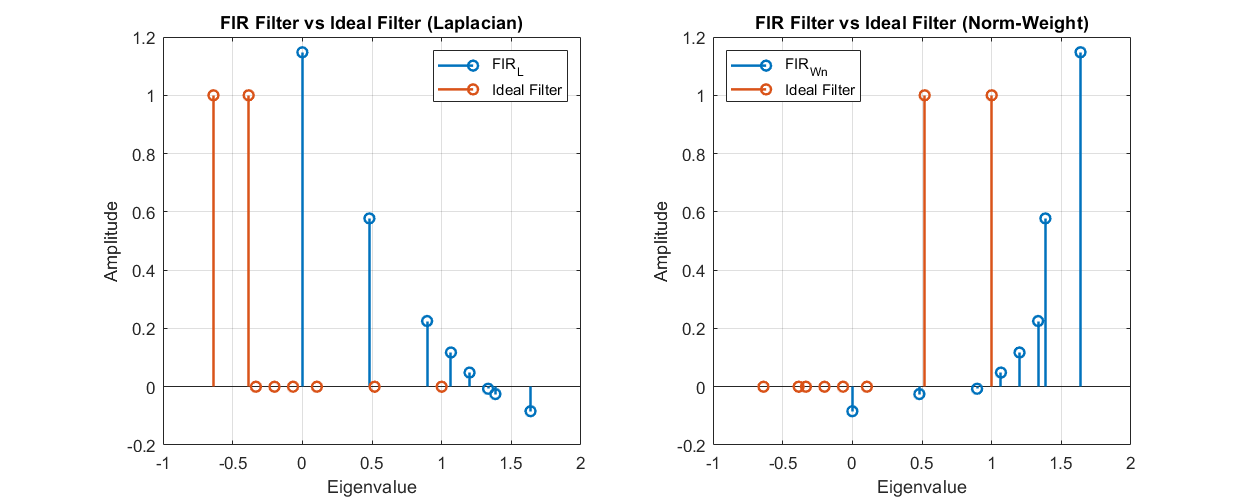
\includegraphics[scale=0.4]{fig10.png} 
        \caption{FIR filters' coeffs with three taps and also the ideal one}
        \label{fig:gr7}
    \end{figure}

    % ---- 
    \item 
    The original signal, the noisy signal, filtered with the Laplacian filter, and filtered with the normalized weight filter. As seen, the SNR in Figures 5, 6 is much better than 7, as expected, with the increase in the FIR filter length, but this difference becomes smaller and smaller.
    \\
    $SNR_{default} = 7.635 \xrightarrow{} SNR_{FIR,L_N} = 13.48 \xrightarrow{} SNR_{FIR,Wn} = 12.3 $\\
    \begin{figure}[h!]
        \centering
        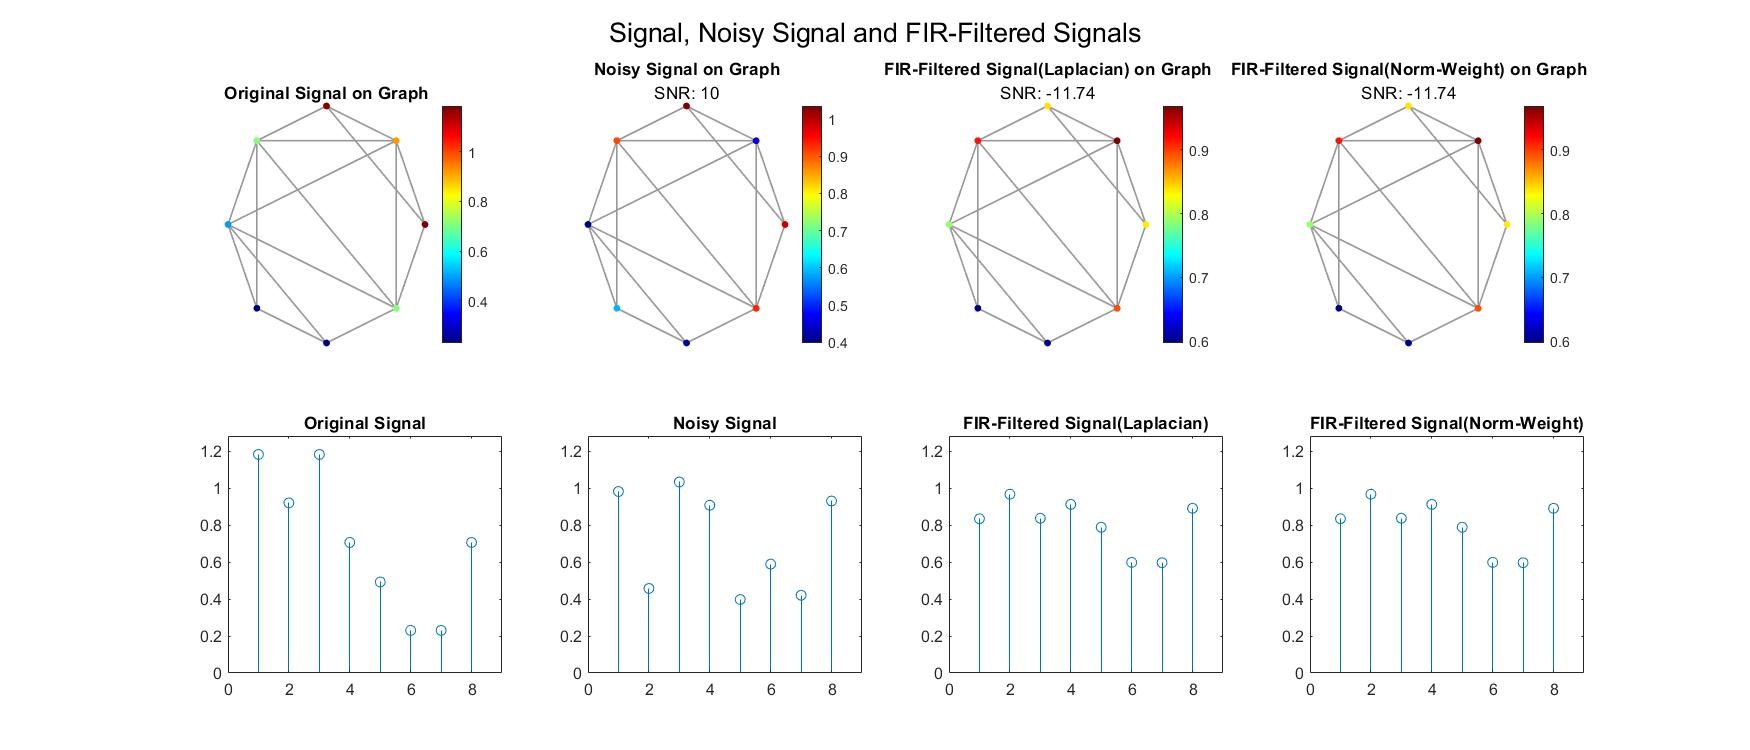
\includegraphics[scale=0.4]{fig11.png} 
        \caption{}
        \label{fig:gr7}
    \end{figure}
    \\
    And the code is put down here:
\begin{lstlisting}
x_FIR_L = U_lap * (FIR_L .* x_n_hat_L);
x_FIR_Wn = U_wn * (FIR_Wn .* x_n_hat_W);

snr_FIR_L = db(snr(x_FIR_L, x));
snr_FIR_Wn = db(snr(x_FIR_Wn, x));

\end{lstlisting}
\end{enumerate}
% --------------------------------------------------
\maketitle
\section*{Problem 2}
\begin{enumerate}
    \item 

    Here is the code for generating the SBM Graph with three clusters:
\begin{lstlisting}
N = 150;
p = 8 * log(N) / N;
q = log(N) / N;
k = 3;
dim = k;

% Generate SBM graph
seed = 20;
rng(seed)
sig = randi([0, k - 1], [N, 1]);
sig = 2 * rescale(sig) - 1;
P = (sig == sig') * p + (sig ~= sig') * q;
A = ones(N) - (rand(N) > P);
A = triu(A);
A = abs(A - A');

% Create graph and compute Fourier basis
G = gsp_graph(A);
G = gsp_create_laplacian(G);
G = gsp_compute_fourier_basis(G);

% Choose subset of Fourier basis for visualization
U23 = G.U;
G.coords = U23(:, 2:max(3, dim));
\end{lstlisting}

    The visualized graph is depicted down below:
    \begin{figure}[h!]
        \centering
        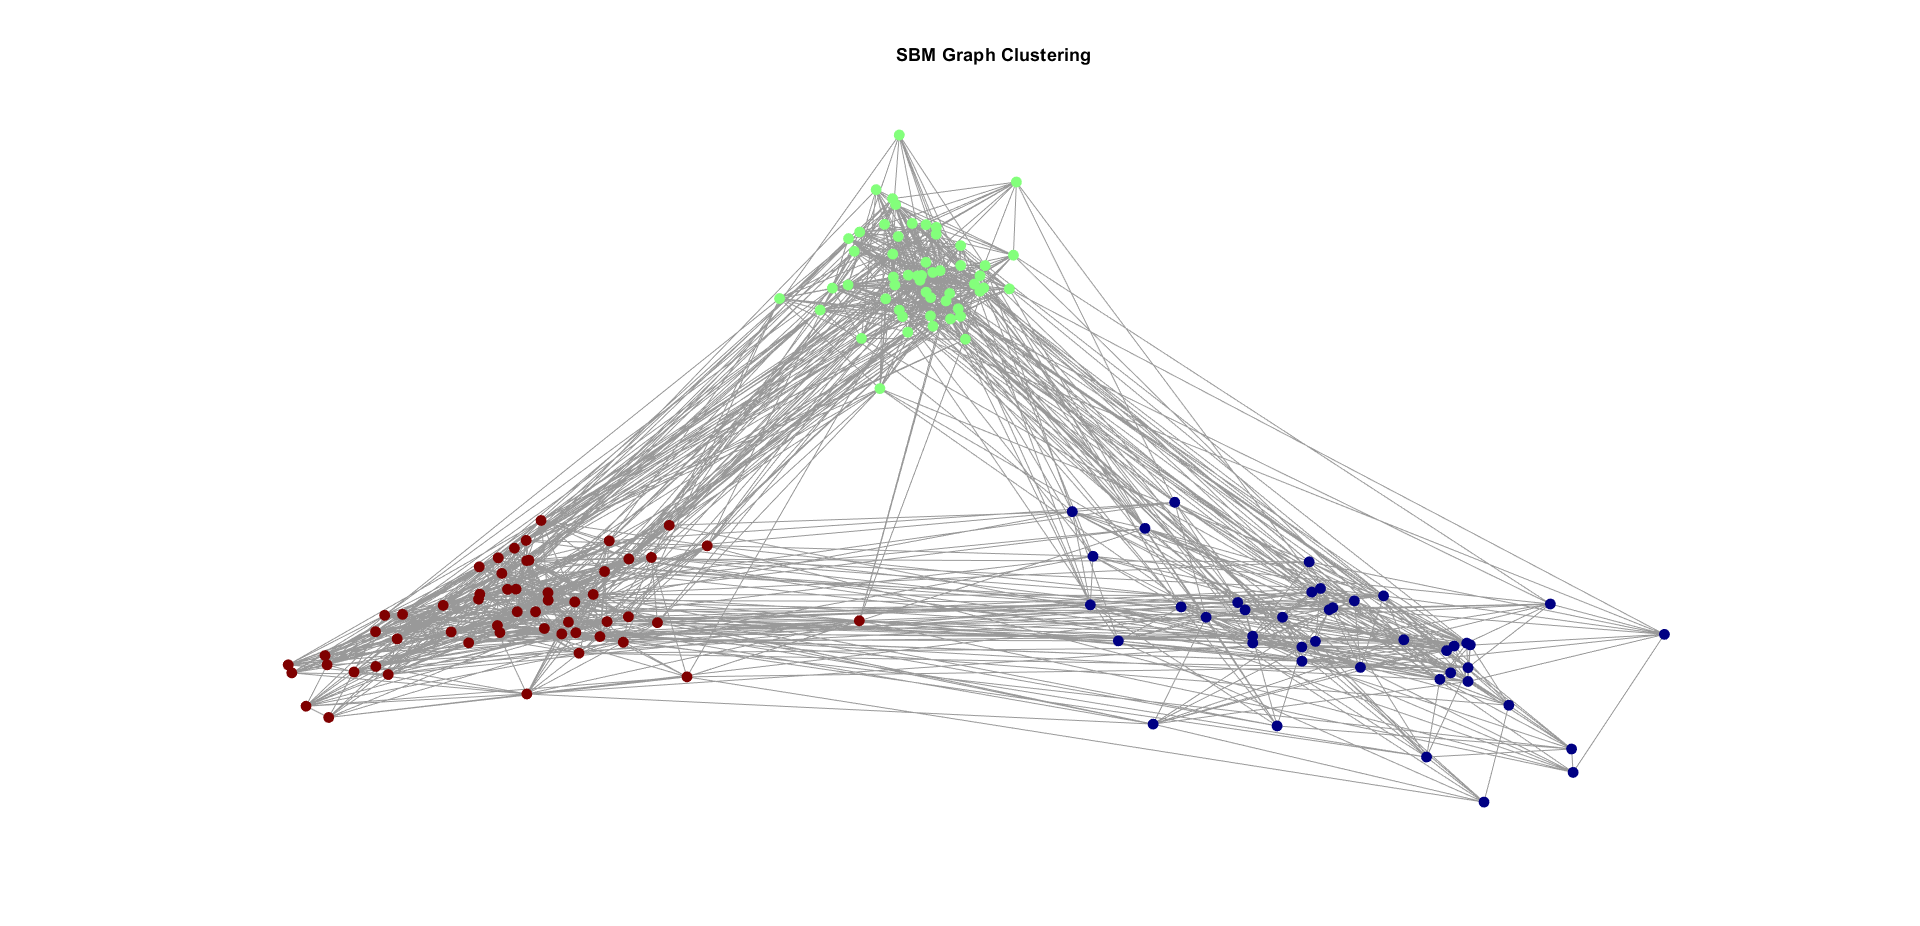
\includegraphics[scale=0.4]{fig12.png} 
        \caption{The SBM graph with three clusters}
        \label{fig:gr8}
    \end{figure}


    % -------------------------
    \newpage
    \item

    Now, using the graph we constructed in the previous section, we generate \( t \) smooth signals using an FIR filter of degree \( r \). Our filter is defined as \( H = (1 -\alpha L_G )^{-r} \), and we pass \( t \) white noise signals through this filter to obtain the smooth signals.
    \\
    As shown in Figure 10, these smooth signals can perform good classification on their own and provide insight into the groupings. Now, we will attempt to use these signals to perform grouping and discover the graph structure.
    \\
    
    \begin{figure}[h!]
        \centering
        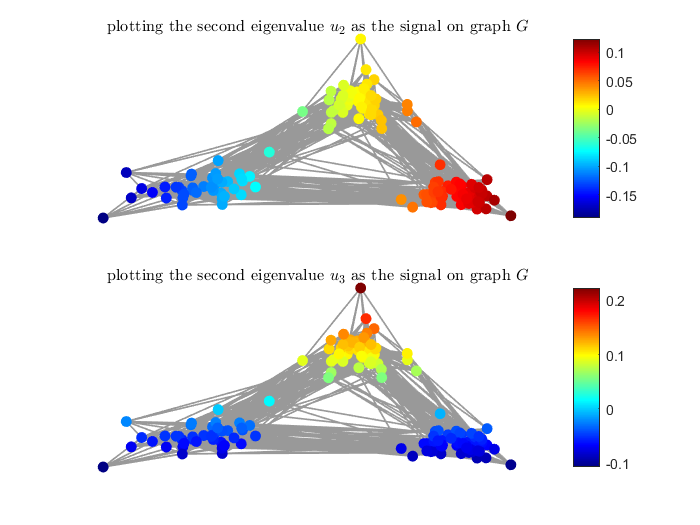
\includegraphics[scale=0.35]{fig13.png} 
        \caption{The eigenvalue signals $u_2, u_3$ on SBM graph}
        \label{fig:gr8}
    \end{figure}
    \\
    And this is the code for generating smooth signals:
\begin{lstlisting}
T = 1000;
r = 31;
X_smooth = gen_smooth(G, T, r);

figure();
gsp_plot_signal(G, X_smooth(:,1), param);
title('Smooth signal on graph');

function x_smooth = gen_smooth_filtered(G, t, r)
    x = randn(G.N, t);
    d_max = max(G.d);
    alpha = 1 / (2 * d_max);
    H = (eye(G.N) - alpha * G.L) ^ (r-1);
    x_smooth = H * x;
end
\end{lstlisting}    

    \begin{figure}[h!]
        \centering
        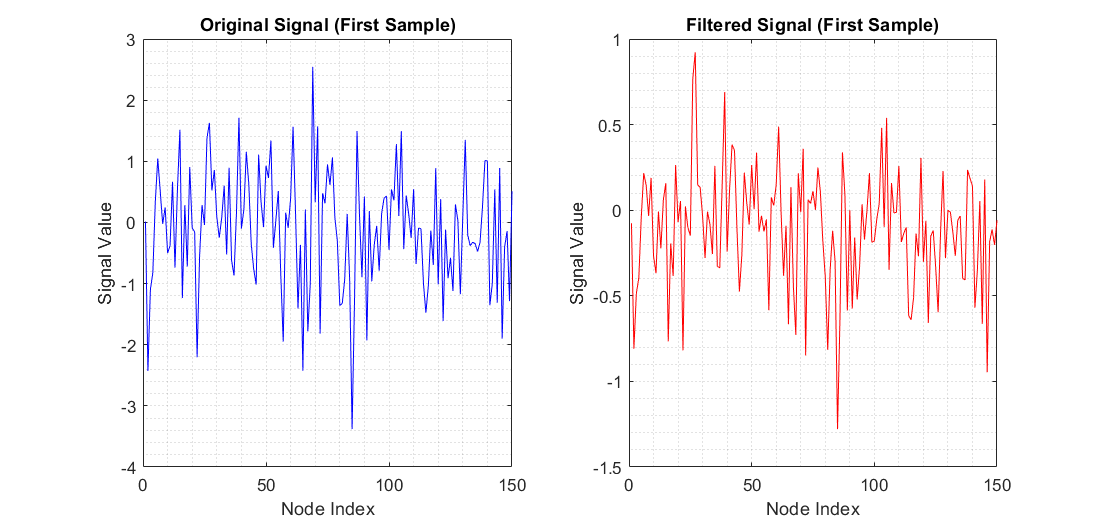
\includegraphics[scale=0.28]{fig14.png} 
        \caption{The time domain on another sight}
        \label{fig:gr9}
    \end{figure}

    \newpage

    This is another visualization, this time on the graph itself:
    \begin{figure}[h!]
    \centering
    \begin{subfigure}{}
        \centering
        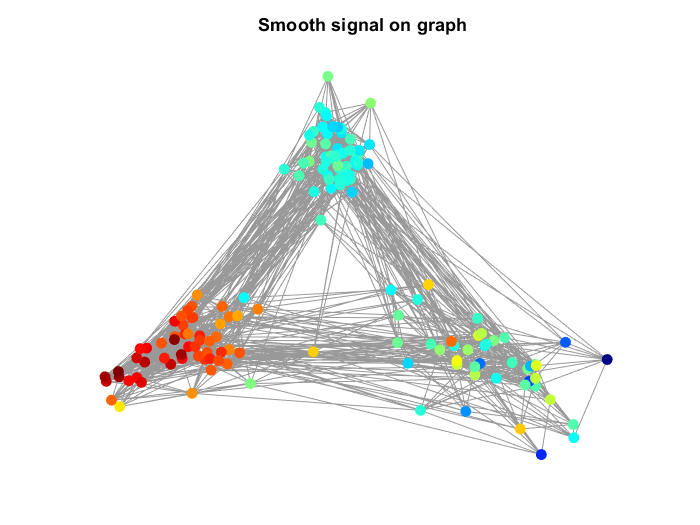
\includegraphics[scale=0.2]{fig16.png}
        \caption{$r=31$}
        \label{fig:r31}
    \end{subfigure}
    %\hfill
    \begin{subfigure}{}
        \centering
        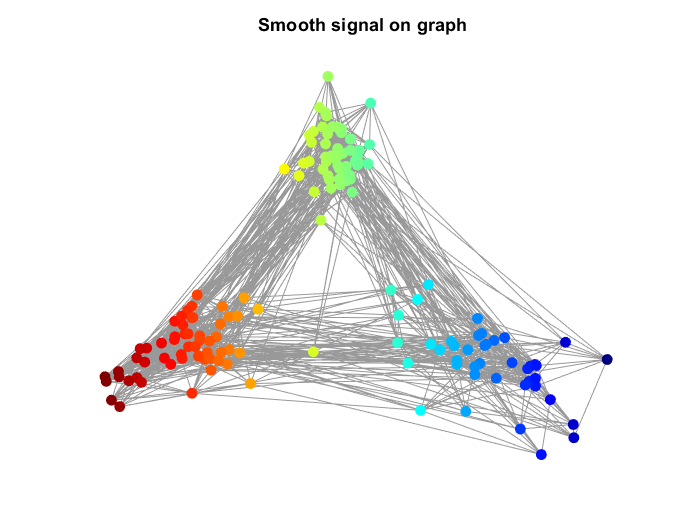
\includegraphics[scale=0.2]{fig17.png}
        \caption{$r=200$}
        \label{fig:r200}
    \end{subfigure}
    %\hfill
    \begin{subfigure}{}
        \centering
        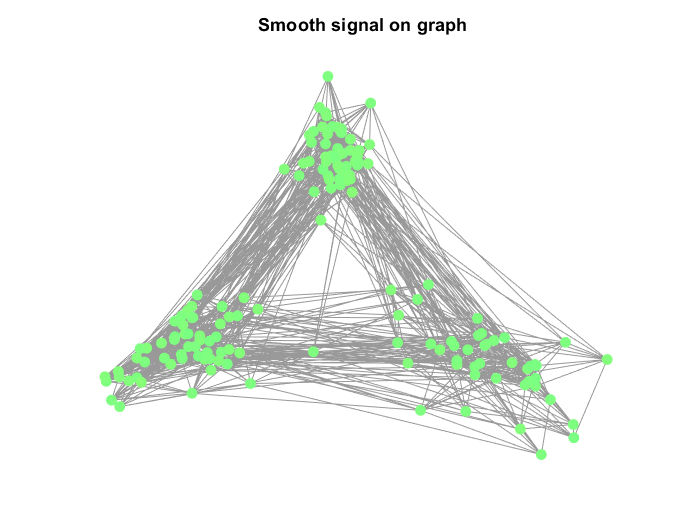
\includegraphics[scale=0.2]{fig18.png}
        \caption{$r=800$}
        \label{fig:r800}
    \end{subfigure}
    \caption{The filtered smooth signal on graph $G$ with $r=31$, $r=200$, and $r=800$, respectively.}
    \label{fig:gr15}
\end{figure}

    The image above shows that, however the graph was random, but we could cluster nodes to some extent. As we can see the value of the filtered signal is roughly the same in each class which shows we were successful!\\ 
    However, increasing $T$ was helpful up to a point, afterwards as you can see, it was destructive and resulted in a uniform filtered signal.

    % -----------------------------------------------
    \item

        
    Random signals \( x \) are generated through a random process and are white Gaussian. The \textbf{spectral density} of this signal is as follows:
    
    \[
    \Sigma_x = I_n = U \sigma^2 U^H = U \text{diag}(1_n) U^H
    \]
    
    \[
    \Sigma_y = U \text{diag}(1_n \cdot |h|^2) U^H = U \text{diag}(|h|^2) U^H = H^2
    \]
    
    \[
    H L = L H
    \]
    
    As a result, the eigenvectors of the covariance matrix are the same as the eigenvectors of the Laplacian matrix. Using this, estimation can be performed. However, we must note that the order of eigenvalues in \( H \) is the reverse of their order in \( L \), and consequently, the order of the signal eigenvectors is also reversed.
    
    After estimating the eigenvectors, the usual steps of \textbf{spectral clustering} are carried out.

    \newpage

    Here are the the results:
    \begin{figure}[h!]
        \centering
        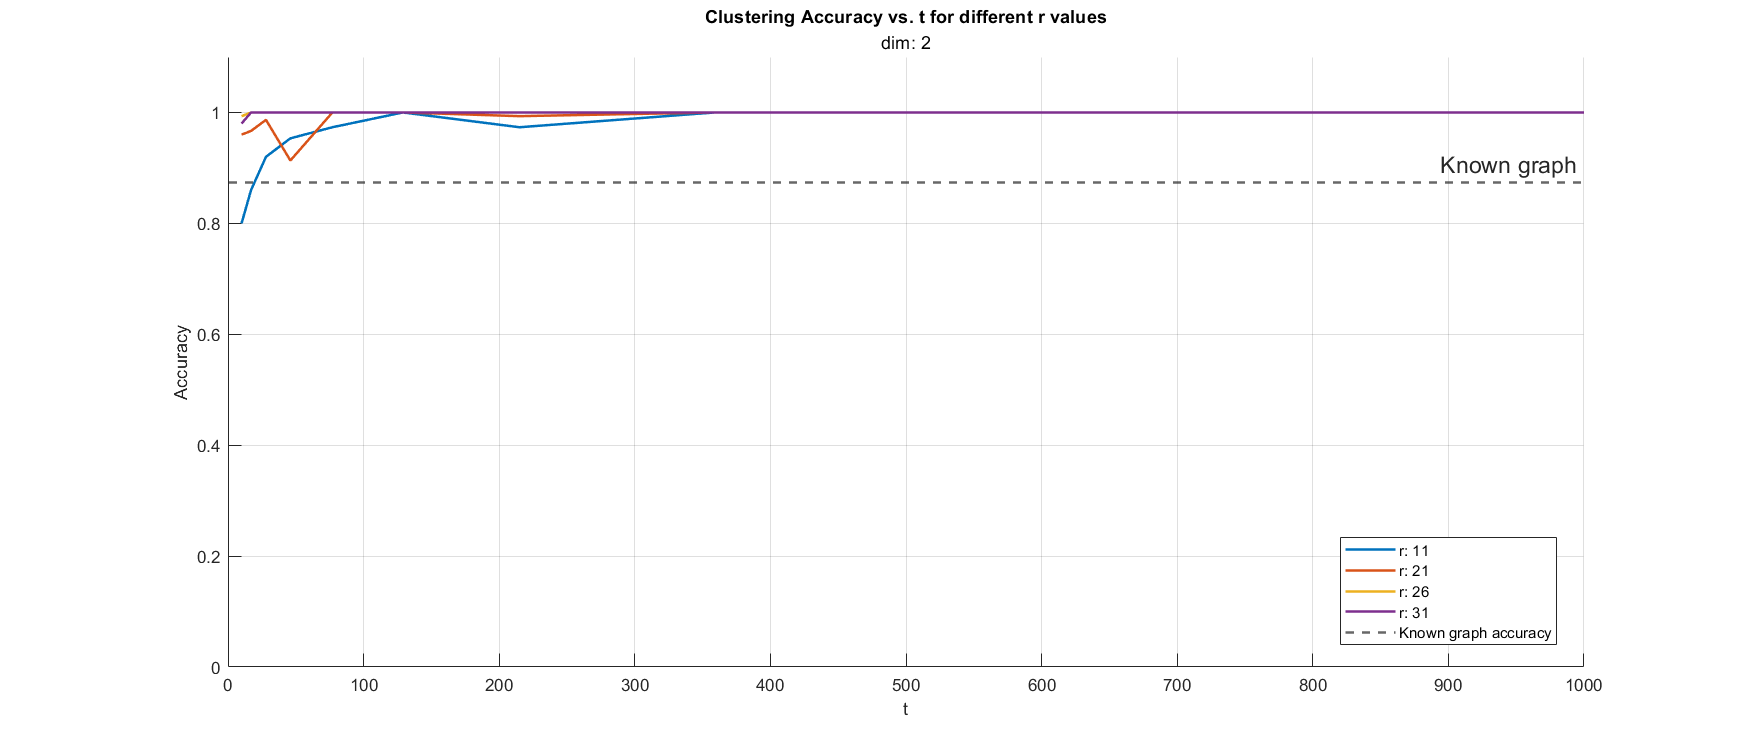
\includegraphics[scale=0.3]{fig15.png} 
        \caption{The time domain on another sight}
        \label{fig:gr16}
    \end{figure}
    
    
    As evident from Figure \( 16 \), this grouping is performed with very high accuracy.  
    
    Using the first two eigenvalues is sufficient. In general, we found that for \( k \)-class classification, using the first \( k-1 \) eigenvectors for embedding is enough.
    
    



    % ------------------------------------
\end{enumerate}
\end{document}
